\title{Machine Learning Spring 2019 HW2}
\author{
        Yueh Cheng Liu \\
        National Taiwain University\\
}
\date{\today}
\documentclass[12pt]{article}
\usepackage{amsmath}
\usepackage{bbm}
\usepackage{graphicx}
\usepackage{mathtools}
\usepackage{bm}
\begin{document}
\maketitle

% \begin{abstract}
% This is the paper's abstraasdsadsct \ldots
% \end{abstract}

\section*{1}

$$
\nabla F(A, B)= 
\begin{bmatrix}
    \frac{\delta F(A, B)}{\delta A}  \\
    \frac{\delta F(A, B)}{\delta B} 
\end{bmatrix}
$$

\begin{equation*}
\begin{split}
    \frac{\delta F(A, B)}{\delta A} &= \frac{1}{N} \sum_{n=1}^N \frac{\delta (-y_n(Az_n + B))}{\delta A} \frac{e^{-y_n(Az_n+B)}}{1+ e^{-y_n(Az_n+B)}} \\
    &= \frac{1}{N} \sum_{n=1}^{N} p_n \frac{\delta (-y_n (Az_n + B))}{\delta A} \\
    &= \frac{1}{N} \sum_{n=1}^{N} -p_ny_nz_n
\end{split}
\end{equation*}
and 
\begin{equation*}
\begin{split}
    \frac{\delta F(A, B)}{\delta B} &= \frac{\delta F(A, B)}{\delta B} \\
    &= \frac{1}{N} \sum_{n=1}^{N} \frac{\delta (-y_n (Az_n + B))}{\delta B} \frac{e^{-y_n(Az_n+B)}}{1+ e^{-y_n(Az_n+B)}} \\
    &= \frac{1}{N} \sum_{n=1}^{N} p_n \frac{\delta (-y_n (Az_n + B))}{\delta B} \\
    &= \frac{1}{N} \sum_{n=1}^{N} -p_ny_n
\end{split}
\end{equation*}


\section*{2}

$$
H(F) = 
\begin{bmatrix}
    \frac{\delta^2 F(A, B)}{\delta A^2} & \frac{\delta^2 F(A, B)}{\delta A \delta B} \\
    \frac{\delta^2 F(A, B)}{\delta B \delta A} & \frac{\delta^2 F(A, B)}{\delta B^2}
\end{bmatrix}
$$
\begin{equation*}
\begin{split}
    \frac{\delta \theta(x)}{\delta x} &= \frac{\delta \frac{e^x}{1+e^x}}{\delta x} \\
    &= \frac{\delta (1+e^{-x})^{-1}}{\delta x} \\
    &= -e^{-x} \cdot -(1+e^{-x})^{-2} \\
    &= \frac{1}{1+e^{-x}} \frac{e^-x}{1+e^{-x}} \\
    &= \theta(x) (1 - \theta(x))
\end{split}
\end{equation*}

\begin{equation*}
    \begin{split}
        \frac{\delta^2 F(A, B)}{\delta A^2} &= \frac{ \delta \frac{1}{N} \sum_{n=1}^N -y_nz_n \theta(-y_n(Az_n+B))}{\delta A} \\
        &= \frac{1}{N} \sum_{n=1}^N -y_nz_n \theta(-y_n(Az_n+B)) (1 - \theta(-y_n(Az_n+B))) \frac{\delta (-y_n (Az_n + B))}{\delta A} \\
        &= \frac{1}{N} \sum_{n=1}^N y_n^2z_n^2 \theta(-y_n(Az_n+B)) (1 - \theta(-y_n(Az_n+B))) \\
        &= \frac{1}{N} \sum_{n=1}^N y_n^2z_n^2 p_n (1-p_n)
    \end{split}
\end{equation*}

\begin{equation*}
    \begin{split}
        \frac{\delta^2 F(A, B)}{\delta B^2} &= \frac{ \delta \frac{1}{N} \sum_{n=1}^N -y_n \theta(-y_n(Az_n+B))}{\delta B} \\
        &= \frac{1}{N} \sum_{n=1}^N y_n^2 \theta(-y_n(Az_n+B)) (1 - \theta(-y_n(Az_n+B))) \\
        &= \frac{1}{N} \sum_{n=1}^N y_n^2 p_n (1-p_n)
    \end{split}
\end{equation*}

\begin{equation*}
    \begin{split}
        \frac{\delta^2 F(A, B)}{\delta A \delta B} = \frac{\delta^2 F(A, B)}{\delta B \delta A} &= \frac{ \delta \frac{1}{N} \sum_{n=1}^N -y_nz_n \theta(-y_n(Az_n+B))}{\delta B} \\
        &= \frac{1}{N} \sum_{n=1}^N y_n^2 z_n\theta(-y_n(Az_n+B)) (1 - \theta(-y_n(Az_n+B))) \\
        &= \frac{1}{N} \sum_{n=1}^N y_n^2 z_n p_n (1-p_n)
    \end{split}
\end{equation*}

\section*{3}


\section*{4}
\[
\bar{g}(x) = -0.25    
\]
\section*{5}

\begin{equation*}
\begin{split}
    (\tilde{y_n} - w^T \tilde{x_n})^2 &= u_n (y_n - w^Tx_n)^2 \\
    &=  (\sqrt{u_n} y_n - \sqrt{u_n}w^Tx_n)^2
\end{split}
\end{equation*}
so that $(\tilde{x_n}, \tilde{y_n}) = (\sqrt{u_n}x_n, \sqrt{u_n}y_n)$

\section*{6}
Let $\epsilon_t$ be the weighted error at step $t$ and $k_t = \sqrt{\frac{1- \epsilon_t}{\epsilon_t}}$. \\
$\epsilon_1 = 0.22$ and $k_1 = \sqrt{\frac{1- \epsilon_1}{\epsilon_1}}$
\begin{equation*}
\begin{split}
    \frac{u_+^{(2)}} {u_-^{(2)}} &= \frac{u_+^{(1)} / k_1 } {u_-^{(1)} * k_1} \\
    &= \frac{1}{k_1^2} = \frac{0.22}{0.78} = 0.282
\end{split}
\end{equation*}

\section*{7}
For integers between $[-M, M]$ has $2M$ interval. $s$ can be $+1$ or $-1$ and $d$ different feature to choose.
Plus the $2$ decision stumps where $g(x)=+1$ and $g(x)=-1$ for all $x$ which are not effected by $d$. 
The number of different decision stump is $2d 2M+2=42$. 
\section*{8}

\section*{9}
% All E_in [0.3175, 0.3175, 0.32, 0.315, 0.33]
% All E_out [0.36, 0.36, 0.36, 0.4, 0.37]
% 3 50.0 0.315
% 0 0.05 0.36
$\lambda = 50.0$ has the minimum $E_{in} = 0.315$

\section*{10}
$\lambda = 0.05, 0.5, 5$ has the minimum $E_{in} = 0.36$

\section*{11}
% All E_in [0.32, 0.32, 0.3175, 0.31, 0.325]
% All E_out [0.36, 0.36, 0.37, 0.4, 0.37]
% 3 50.0 0.31
% 0 0.05 0.36
$\lambda = 50.0$ has the minimum $E_{in} = 0.31$

\section*{12}
$\lambda = 0.05, 0.5$ has the minimum $E_{in} = 0.36$

\section*{13}
\begin{center}
    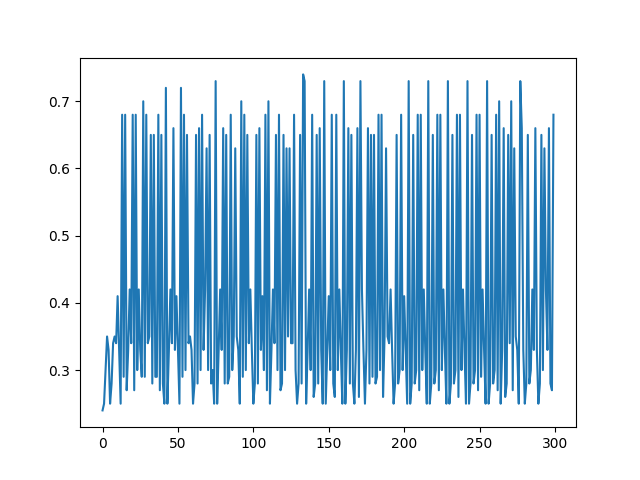
\includegraphics[scale=0.5]{p13.png}
\end{center}
$E_{in}(g_T) = 0.65$. The $E_{in}(g_t)$ is bouncing.
\section*{14}
\begin{center}
    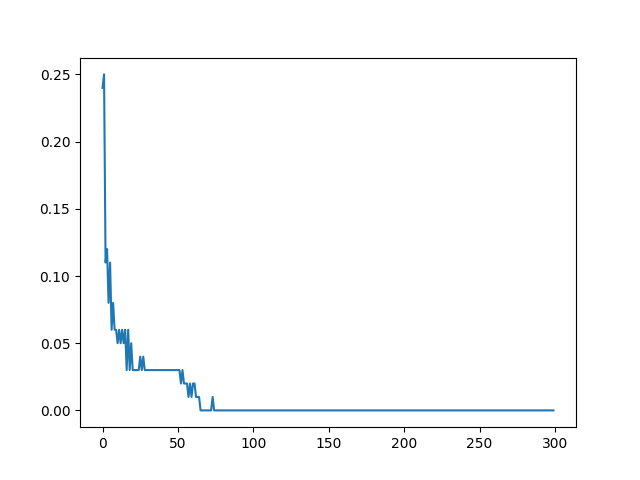
\includegraphics[scale=0.5]{p14.png}
\end{center}
$E_{in}(G_T) = 0$. The $E_{in}(G_t)$ decreases to $0$ before step $50$.

\section*{15}
\begin{center}
    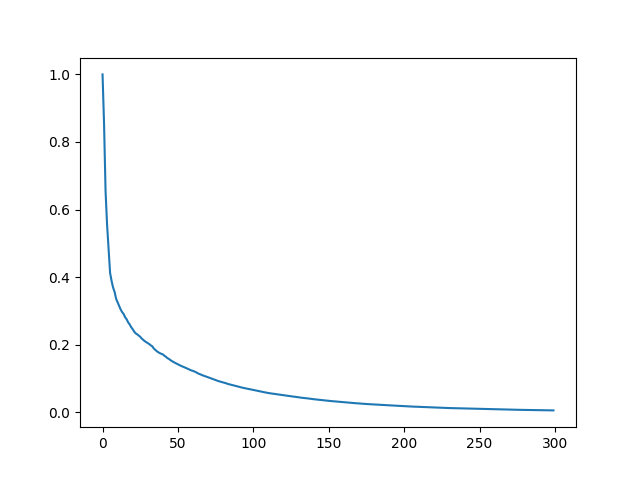
\includegraphics[scale=0.5]{p15.png}
\end{center}
$U_T \simeq 0$

\section*{16}
\begin{center}
    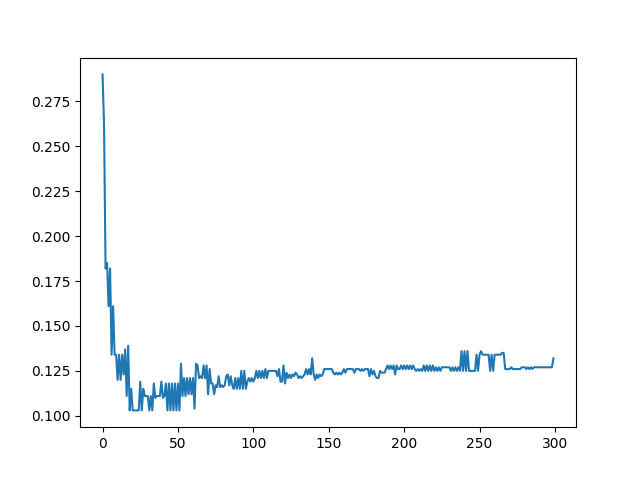
\includegraphics[scale=0.5]{p16.png}
\end{center}
$E_{out}(G_T) = 0.212$
\section*{17}

\section*{18}


\end{document}


